% Options for packages loaded elsewhere
% Options for packages loaded elsewhere
\PassOptionsToPackage{unicode}{hyperref}
\PassOptionsToPackage{hyphens}{url}
\PassOptionsToPackage{dvipsnames,svgnames,x11names}{xcolor}
%
\documentclass[
  12pt,
]{article}
\usepackage{xcolor}
\usepackage[margin=2cm]{geometry}
\usepackage{amsmath,amssymb}
\setcounter{secnumdepth}{5}
\usepackage{iftex}
\ifPDFTeX
  \usepackage[T1]{fontenc}
  \usepackage[utf8]{inputenc}
  \usepackage{textcomp} % provide euro and other symbols
\else % if luatex or xetex
  \usepackage{unicode-math} % this also loads fontspec
  \defaultfontfeatures{Scale=MatchLowercase}
  \defaultfontfeatures[\rmfamily]{Ligatures=TeX,Scale=1}
\fi
\usepackage{lmodern}
\ifPDFTeX\else
  % xetex/luatex font selection
  \setmainfont[]{Times New Roman}
\fi
% Use upquote if available, for straight quotes in verbatim environments
\IfFileExists{upquote.sty}{\usepackage{upquote}}{}
\IfFileExists{microtype.sty}{% use microtype if available
  \usepackage[]{microtype}
  \UseMicrotypeSet[protrusion]{basicmath} % disable protrusion for tt fonts
}{}
\makeatletter
\@ifundefined{KOMAClassName}{% if non-KOMA class
  \IfFileExists{parskip.sty}{%
    \usepackage{parskip}
  }{% else
    \setlength{\parindent}{0pt}
    \setlength{\parskip}{6pt plus 2pt minus 1pt}}
}{% if KOMA class
  \KOMAoptions{parskip=half}}
\makeatother
% Make \paragraph and \subparagraph free-standing
\makeatletter
\ifx\paragraph\undefined\else
  \let\oldparagraph\paragraph
  \renewcommand{\paragraph}{
    \@ifstar
      \xxxParagraphStar
      \xxxParagraphNoStar
  }
  \newcommand{\xxxParagraphStar}[1]{\oldparagraph*{#1}\mbox{}}
  \newcommand{\xxxParagraphNoStar}[1]{\oldparagraph{#1}\mbox{}}
\fi
\ifx\subparagraph\undefined\else
  \let\oldsubparagraph\subparagraph
  \renewcommand{\subparagraph}{
    \@ifstar
      \xxxSubParagraphStar
      \xxxSubParagraphNoStar
  }
  \newcommand{\xxxSubParagraphStar}[1]{\oldsubparagraph*{#1}\mbox{}}
  \newcommand{\xxxSubParagraphNoStar}[1]{\oldsubparagraph{#1}\mbox{}}
\fi
\makeatother


\usepackage{longtable,booktabs,array}
\usepackage{calc} % for calculating minipage widths
% Correct order of tables after \paragraph or \subparagraph
\usepackage{etoolbox}
\makeatletter
\patchcmd\longtable{\par}{\if@noskipsec\mbox{}\fi\par}{}{}
\makeatother
% Allow footnotes in longtable head/foot
\IfFileExists{footnotehyper.sty}{\usepackage{footnotehyper}}{\usepackage{footnote}}
\makesavenoteenv{longtable}
\usepackage{graphicx}
\makeatletter
\newsavebox\pandoc@box
\newcommand*\pandocbounded[1]{% scales image to fit in text height/width
  \sbox\pandoc@box{#1}%
  \Gscale@div\@tempa{\textheight}{\dimexpr\ht\pandoc@box+\dp\pandoc@box\relax}%
  \Gscale@div\@tempb{\linewidth}{\wd\pandoc@box}%
  \ifdim\@tempb\p@<\@tempa\p@\let\@tempa\@tempb\fi% select the smaller of both
  \ifdim\@tempa\p@<\p@\scalebox{\@tempa}{\usebox\pandoc@box}%
  \else\usebox{\pandoc@box}%
  \fi%
}
% Set default figure placement to htbp
\def\fps@figure{htbp}
\makeatother





\setlength{\emergencystretch}{3em} % prevent overfull lines

\providecommand{\tightlist}{%
  \setlength{\itemsep}{0pt}\setlength{\parskip}{0pt}}



 


\usepackage{booktabs}
\usepackage{longtable}
\usepackage{array}
\usepackage{multirow}
\usepackage{wrapfig}
\usepackage{float}
\usepackage{colortbl}
\usepackage{pdflscape}
\usepackage{tabu}
\usepackage{threeparttable}
\usepackage{threeparttablex}
\usepackage[normalem]{ulem}
\usepackage{makecell}
\usepackage{xcolor}
\makeatletter
\@ifpackageloaded{caption}{}{\usepackage{caption}}
\AtBeginDocument{%
\ifdefined\contentsname
  \renewcommand*\contentsname{Table of contents}
\else
  \newcommand\contentsname{Table of contents}
\fi
\ifdefined\listfigurename
  \renewcommand*\listfigurename{List of Figures}
\else
  \newcommand\listfigurename{List of Figures}
\fi
\ifdefined\listtablename
  \renewcommand*\listtablename{List of Tables}
\else
  \newcommand\listtablename{List of Tables}
\fi
\ifdefined\figurename
  \renewcommand*\figurename{Figure}
\else
  \newcommand\figurename{Figure}
\fi
\ifdefined\tablename
  \renewcommand*\tablename{Table}
\else
  \newcommand\tablename{Table}
\fi
}
\@ifpackageloaded{float}{}{\usepackage{float}}
\floatstyle{ruled}
\@ifundefined{c@chapter}{\newfloat{codelisting}{h}{lop}}{\newfloat{codelisting}{h}{lop}[chapter]}
\floatname{codelisting}{Listing}
\newcommand*\listoflistings{\listof{codelisting}{List of Listings}}
\makeatother
\makeatletter
\makeatother
\makeatletter
\@ifpackageloaded{caption}{}{\usepackage{caption}}
\@ifpackageloaded{subcaption}{}{\usepackage{subcaption}}
\makeatother
\usepackage{bookmark}
\IfFileExists{xurl.sty}{\usepackage{xurl}}{} % add URL line breaks if available
\urlstyle{same}
\hypersetup{
  pdftitle={Supplementary material},
  colorlinks=true,
  linkcolor={blue},
  filecolor={Maroon},
  citecolor={Blue},
  urlcolor={Blue},
  pdfcreator={LaTeX via pandoc}}


\title{Supplementary material}



\date{}
\begin{document}
\maketitle


\section{Correlation matrix}\label{correlation-matrix}

\begin{figure}

\caption{\label{fig-cr}Correlation matrix for the pooled sample}

\centering{


\includegraphics[width=0.8\linewidth,height=\textheight,keepaspectratio]{07-supplementary-material_files/figure-pdf/fig-cr-1.pdf}

}

\end{figure}%

\newpage{}

\section{Confirmatory factor analysis of the meritocracy
scale}\label{confirmatory-factor-analysis-of-the-meritocracy-scale}

\begin{figure}

\caption{\label{fig-w1}CFA model for the first wave}

\centering{

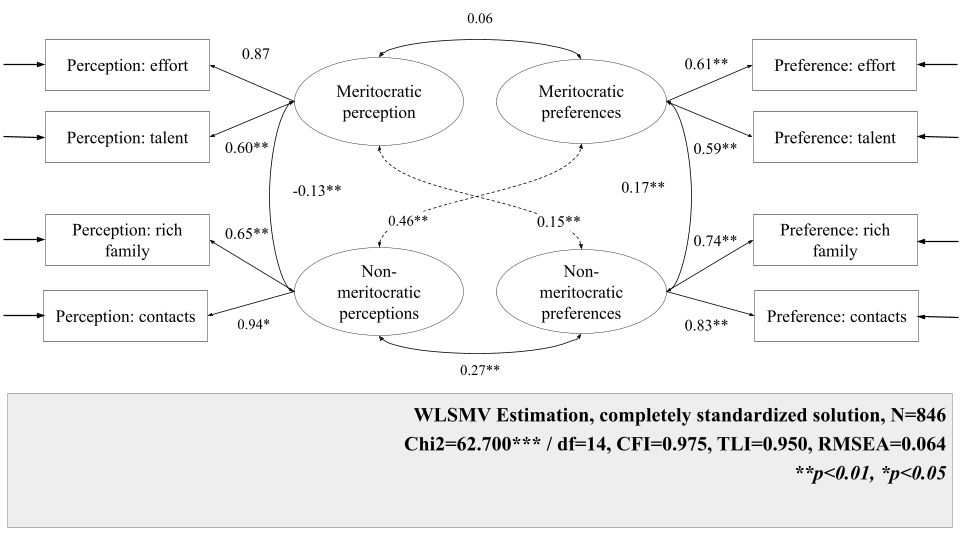
\includegraphics[width=0.8\linewidth,height=\textheight,keepaspectratio]{imagenes/w1.png}

}

\end{figure}%

\begin{figure}

\caption{\label{fig-w2}CFA model for the second wave}

\centering{

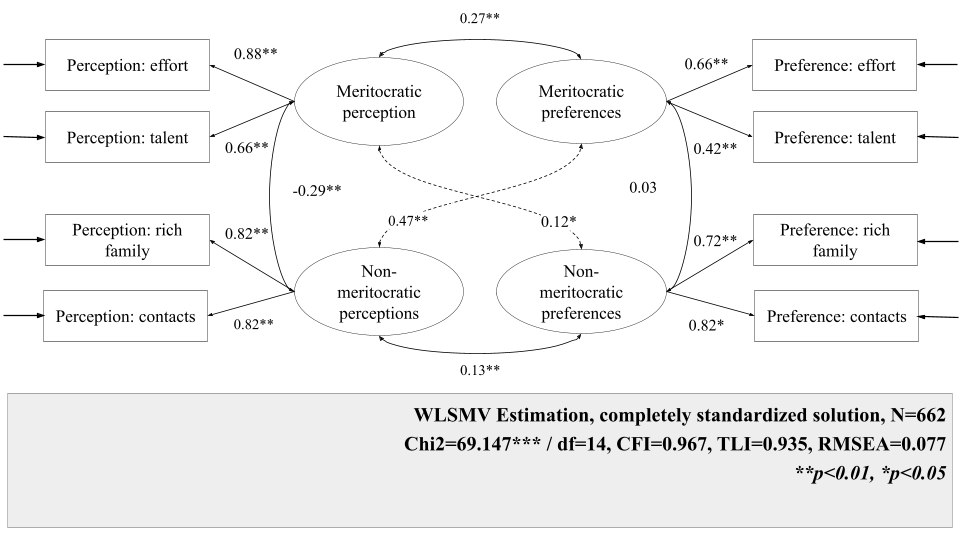
\includegraphics[width=0.8\linewidth,height=\textheight,keepaspectratio]{imagenes/w2.png}

}

\end{figure}%

\begin{figure}

\caption{\label{fig-basica}CFA model for the primary cohort}

\centering{

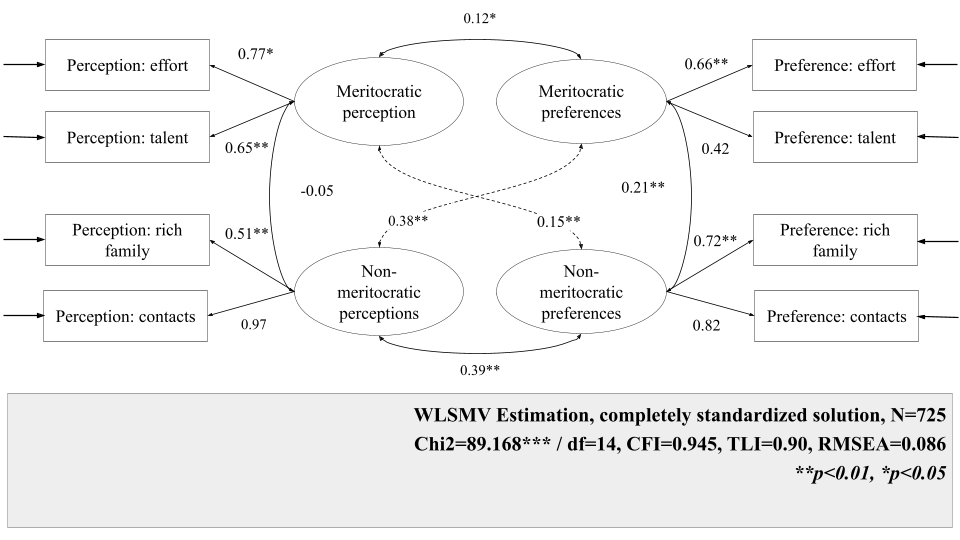
\includegraphics[width=0.8\linewidth,height=\textheight,keepaspectratio]{imagenes/basica.png}

}

\end{figure}%

\begin{figure}

\caption{\label{fig-media}CFA model for the secondary cohort}

\centering{

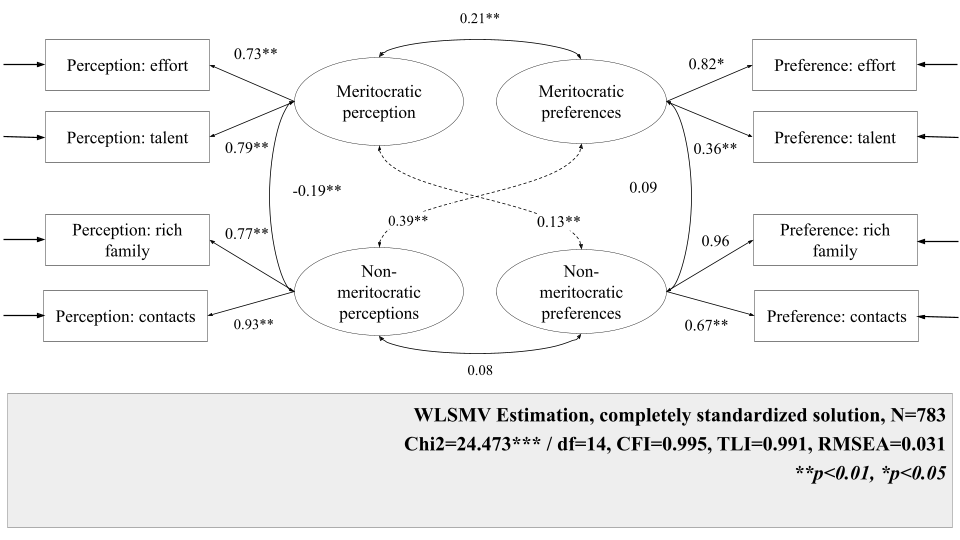
\includegraphics[width=0.8\linewidth,height=\textheight,keepaspectratio]{imagenes/media.png}

}

\end{figure}%

\newpage{}

\section{Sources of misfit in longitudinal
invariance}\label{sources-of-misfit-in-longitudinal-invariance}

For the longitudinal strict invariance model (the more strict model),
score tests provided no evidence of localized misfit. The global score
test was non-significant, \(\chi^2 (20)=11.93, p=.918\), and none of the
univariate score tests for equality constraints was significant (all
\(p>.05\); smallest \(p=.065\)). This indicates that no single equality
constraint notably contributed to the misfit. There are also no
indicators of possible sources of misfit in the previous nested models
(weak and strong).

\newpage{}

\section{Sources of misfit between cohort
invariance}\label{sources-of-misfit-between-cohort-invariance}

In contrast, score tests for the cross-cohort invariance constraints
indicated localized misfit. The largest modification indices/score
contributions clustered in the perceived effort, suggesting that
equality constraints on thresholds/loadings for these items are not
supported across school levels. Table~\ref{tbl-lavtestcohort} lists the
ten constraints with the largest score statistics.

\begin{table}

\caption{\label{tbl-lavtestcohort}Sources of misfit in longitudinal
invariance}

\centering{

\begingroup\fontsize{10}{12}\selectfont

\begin{tabu} to \linewidth {>{\centering}X>{\centering}X>{\centering}X>{\centering}X>{\centering}X>{\centering}X}
\toprule
Item & Threshold & $\chi^2$ & df & p-value & p-value adjustement BH\\
\midrule
Perception effort & t2 & 10.115134 & 1 & 0.0014706 & 0.0352936\\
Perception effort & t1 & 7.546618 & 1 & 0.0060123 & 0.0721474\\
Perception contact & t1 & 5.179947 & 1 & 0.0228490 & 0.1464457\\
Preference effort & t2 & 5.012861 & 1 & 0.0251597 & 0.1464457\\
Perception talent & t1 & 4.680351 & 1 & 0.0305095 & 0.1464457\\
\addlinespace
Perception rich parents & t1 & 3.516226 & 1 & 0.0607707 & 0.2430828\\
Preference effort & t3 & 2.177777 & 1 & 0.1400165 & 0.4800567\\
Perception rich parents & t2 & 1.697639 & 1 & 0.1925971 & 0.5332262\\
Perception talent & t3 & 1.642668 & 1 & 0.1999598 & 0.5332262\\
Perception effort & t3 & 1.026312 & 1 & 0.3110265 & 0.7233287\\
\bottomrule
\end{tabu}
\endgroup{}

}

\end{table}%

\newpage{}

\section{Conditional longitudinal invariance by
cohort}\label{conditional-longitudinal-invariance-by-cohort}

Despite the lack of cohort measurement invariance, we examined whether
plausible cohort-related heterogeneity could compromise longitudinal
invariance by re-estimating the longitudinal invariance sequence while
controlling for cohort (dummy-coded) as a covariate predicting each
latent factor (see Table~\ref{tbl-conditional}). Model fit remained good
across all steps---from the configural baseline to the strict
model---and consistently met conventional standards; for instance, the
strict invariance model with cohort control showed \(\chi^2\)(92) =
131.64, CFI = .991, and RMSEA = .027. Importantly, including cohort as a
predictor did not materially alter model fit or the invariance
conclusions, suggesting that the equality constraints over time are
tenable even after accounting for cohort differences in average latent
factor levels.

\begin{table}

\caption{\label{tbl-conditional}Conditional longitudinal invariance by
cohort level}

\centering{

\begingroup\fontsize{9.5}{11.5}\selectfont

\begin{tabu} to \linewidth {>{\centering\arraybackslash}p{2cm}>{\centering}X>{\centering}X>{\centering\arraybackslash}p{2 cm}>{\centering}X>{\centering}X>{\centering}X>{\centering}X}
\toprule
Model & $\chi^2$ (df) & CFI & RMSEA (90\% CI) & $\Delta \chi^2$ ($\Delta$df) & $\Delta$CFI & $\Delta$RMSEA & Decision\\
\midrule
Configural & 122.27 (76) & 0.990 & 0.032 
 (0.021-0.042) & 0 (0) & 0.000 & 0.000 & Reference\\
Weak & 126.95 (80) & 0.990 & 0.032 
 (0.021-0.042) & 4.684 (4) & 0.000 & -0.001 & Accept\\
Strong & 128.55 (88) & 0.991 & 0.028 
 (0.017-0.038) & 1.598 (8) & 0.001 & -0.004 & Accept\\
Strict & 131.64 (92) & 0.991 & 0.027 
 (0.016-0.037) & 3.086 (4) & 0.000 & -0.001 & Accept\\
\bottomrule
\end{tabu}
\endgroup{}

}

\end{table}%

This result has two main implications. First, it strengthens the claim
that the measurement properties of the scale are temporally stable
within individuals: observed over-time comparisons are not driven by
shifts in how primary versus secondary students use the response
categories, but reflect stability (or change) in the underlying latent
constructs. Second, it clarifies the scope of the cohort non-invariance
finding. Non-invariance across cohorts appears to be primarily a
cross-sectional comparability problem---limiting direct comparisons of
latent means or observed scores between educational levels at a given
wave---rather than a threat to longitudinal analyses pooling both
cohorts. Therefore, analyses of within-person change and over-time
associations can be interpreted with greater confidence, while cohort
contrasts should be treated cautiously (or handled via partial
invariance, alignment, or cohort-specific models).




\end{document}
